\section{Foreword}
In $2007$ I began to write some of MicMac documentation in French. Then,
for different reasons (laziness, lack of courage, idleness, \dots) I stopped.

In March $2011$, as preparing a course on my photogrammetric tools, I decided
to start again this documentation. I thought it would be useful to
do it in a language (hopefully) close to English.  This is the new
version you are reading. However, I doubt that it may be complete before a long time and,
during this transitional step, I will conserve the existing French chapter at the end
of this documentation and there may be some cross references between English and French chapters.



\chapter{Introduction}


%=======================================================================================================
\section{History, Status and Contributors}

This is the documentation of a set of software
photogrammetric tools that, under certain
conditions, allow to compute a 3D modelization from a
set of images.

MicMac is a tool for image matching. I began to write it in $2005$, while working at the
French National Geographic Institute (IGN), as
a tool integrating several recent results of the scientific community.
It is a general purpose tool, probably in many (if not all) specific
contexts, one will be able to find a more accurate tool. However, one
of its expected advantages is its generality. It has been used
in a lot of different contexts, for example:

\begin{itemize}
   \item digital terrain model in rural context from pairs of satellite
         images, with exact or approximate orientation;

   \item digital elevation model in urban context with high resolution
         multi-stereoscopic images;

   \item detection of terrain movements;

   \item 3D modelization of objects (sculptures) or interior and exterior scenes;

   \item multi-spectral matching of images registration.

\end{itemize}

Of course this generality comes with a price \dots : it requires a lot of parameterization
which sometimes turns to be quite complex.  For 3D computation, MicMac works only
with oriented images like the ones resulted from classical aero-triangulation process. Early
in $2007$, there were several opportunities that encouraged me to create a
tool that could orientate a set of overlapping images, so that they can be matched in
MicMac:

\begin{itemize}
   \item  I bought my first reflex digital camera, and thought it would be fun
          to be able to make 3D models from my holidays pictures, which turned to be right;

   \item  I discovered the existence of the magical SIFT algorithm from David Lowe, and thought this
          would make this idea feasible by solving the tie point problem, which turned to be right;

   \item  I had already written several pieces of software, including some calibration tools, which
          could be reused and made me think it could be done easily and quickly, which turned to be wrong \dots
\end{itemize}

Since $2008$, several tools were added to solve specific requirements: tools for ortho-photo, tools
for demosaicing\dots \  Since $2007$,  MicMac is an open source software, under the CeCILL-B license
(an adaptation to the French law of the L-GPL license); as far as I understand law (not very much) all
the other tools described in this document are extensions and evolutions of MicMac and obey to
the same license.

Different people have helped me in writing these tools:

\begin{itemize}
   \item Gregoire Maillet for supporting satellite orientation models (grid of rpc),
   \item Arnaud Le Bris for adaptation of \SiftPP supporting large images,
   \item Didier Boldo for the first Windows adaptation,
   \item Aymeric Godet and Livio de Luca for  developing two different user friendly interfaces and also making many tests,
   \item Christophe Meynard for solving some tricky Linux problems,
   \item Christian Thom for the first idea of multi-correlation,
   \item Jean-Micha\"el Muller for improvements about installation,
   \item Ana-Maria Rosu for many typo corrections (alas, I can create them faster than she can correct them).
   \item since september $2012$, the \emph{culture 3D} team : J\'er\'emie Belvaux, G\'erald Choqueux,
         Matthieu Deveau.
\end{itemize}

Of course, there are also many people who helped without knowing by creating
free softwares which I integrated:


\begin{itemize}
   \item    AMD  (\url{http://www.cise.ufl.edu/research/sparse/amd/}) for approximate minimum degree ordering;
   \item    SIFT
   \item    DCRAW by Dave Coffin ( \url{http://www.cybercom.net/~dcoffin/dcraw/}) for using raw image;
   \item    image magick for convert, for using jpg images (\url{http://www.imagemagick.org/});
   \item    proj4 for handling cartographic projection (\url{http://trac.osgeo.org/proj/}) ;
\end{itemize}


%===========================================================================
\section{Prerequisites}

These tools are low-level tools. Although I will try to make this
documentation as clear and self-contained as possible, there are some
prerequisites:

\begin{itemize}
   \item the reader must be comfortable with the Linux PC on which the software
         will be installed; at least, if you are not familiar with installation
         of software from source code, you should have the support of
         an administrator;

   \item some very basic notions of photogrammetry are necessary, not a lot
         (for example to have a notion of what cross-correlation,
         epipolar geometry, rotation matrix are).
\end{itemize}


%=======================================================================================================
\section{Installation and Distribution}

\subsection{Documentation}

This document is rather a "reference" documentation, not specially tuned for an
easy begining; for reference to photogrammetry with MicMac see :

\begin{itemize}
   \item \url{http://jmfriedt.free.fr/lm\_sfm\_eng.pdf} by JM Friedt;
   \item \url{http://forum-micmac.forumprod.com/bibliography-f38.html} a section of the forum dedicated to bibliography;
   \item several documents in the {\tt Documentation} folder and sub folder of MicMac distribution (see in
         particular {\tt pdf} file
         and {\tt Paper-Algo/ , Paper-MPD/ , Papers-Internship/ , Paper-UseCase/} sub folder)
   \item \href{http://combiencaporte.blogspot.fr/2013/10/micmac-tutoriel-de-photogrammetrie-sous.html}{micmac-tutoriel-de-photogrammetrie}\\*
\end{itemize}



There is also a forum where you will find answers to the most frequent question
you may have : \url{http://forum-micmac.forumprod.com/}



\subsection{Install}

\label{Install}
These tools are written in \CPP. They are distributed mainly in source code
format that you have to compile. As described below, they are relatively
low level tools, and the installation, computation and running of these
tools require some basic background in practical computer science.

See now the section~\ref{MERCURIAL} for the new website since $2012$, install mercurial and follow the instruction.
Several links that may be useful :

\begin{itemize}
   \item \url{http://logiciels.ign.fr/?Telechargement,20}   for the sources
   \item \url{http://forum-micmac.forumprod.com/new-site-of-micmac-since-januray-2013-t340.html}
   \item \url{http://forum-micmac.forumprod.com/tuto-install-t518.html}
\end{itemize}


In this documentation, you will find examples that require some
data.The server is now a {\tt ftp} server :

\begin{verbatim}

ftp2.ign.fr
user = micmac_user
pwd = scAEf9MR

\end{verbatim}




%=======================================================================================================

\section{Libraries, Programs and Dependencies}

These softwares have few dependencies to other libraries or programs. Basically,
if you use tiff or raw files as input, and if you do not use any of the graphical
tools provided \footnote{for handling mask, visualize tie points ...} ,
there might not be any dependency.

By the way, on Linux, as the graphical interface are by default required, the compiler
will require the header file {\tt X.h, Xlib.h, Xutil.h, cursorfont.h, keysym.h}.
If they are not installed, you can easily get them  with something like :


\begin{verbatim}
sudo apt-get install x11proto-core-dev libx11-dev
\end{verbatim}

Most users will want sooner or later to use jpeg files. In this case, it will be necessary
to have installed the command {\tt convert}, this command is a part of the excellent
{\tt ImageMagick} package.


The {\tt dcraw} source code I use to handle xif files info is sufficient in most cases.
However, when it fails, I try to use the {\tt exiv2} tool. I also recommend that
you install this excellent and free package.

I also recommend that you install the excellent package {\tt exiftool}, it is a free
open source package and has the ability to read many {\tt xif} information (including
GPS tags that will be soon usable in {\tt Apero}).




%=======================================================================================================
\section{Interface for the Tools}

\subsection{Kinds of Interfaces}
There are roughly three kinds of interfaces for softwares:

\begin{itemize}
   \item user friendly graphical interface, with intuitive menu and window etc.
         Its advantage is that it may be usable by all final users,
         the drawback of this solution being the cost for the developer;

   \item API or application programming interface. Using this level of interface requires you
         to use one of the programming language the API is functioning with. One of
         the drawbacks of these API is that they require a lot of documentation;

   \item a set of programs that you can call on a command line, with parameters being
         added on a command line or included in a file.

\end{itemize}

The tools described here use mainly the third kind of interface. This seemed to be the
optimal solution as these tools have been primarily developed for my own usage and
usage of colleagues from the same building. Since this is not optimal for end users, some user friendly graphical interfaces have been added, to help to set parameters.

\subsection{Simple Tools}

The tools described here are all command line tools. Their parameters can be added
directly on the command line or, for more complex tools (like Apero and MicMac) the
parameters are provided in an XML file.

Here is an example of calling the command {\tt GrShade} for computing the shading
of a depth image:

\begin{verbatim}
bin/GrShade ../micmac_data/Boudha/F050_IMG_5571_MpDcraw8B_GB.tif Visu=1 FZ=0.1
\end{verbatim}

The simple tools described here, that have all their parameters on command lines,
include:

\begin{itemize}
    \item {\tt bin/GrShade} for computing shading;
    \item {\tt bin/Nuage2Ply} for transforming depth map in cloud point in ply format;
    \item {\tt bin/ScaleIm} for rescaling an image (\UNCLEAR{with some care on} aliasing); %dealing with
    \item {\tt bin/ScaleNuage} for scaling a depth map.
\end{itemize}

Generally, these tools understand the syntax {\tt bin/Tool -help} that prints the syntactic
description of the command. For example{ \tt bin/Nuage2Ply -help} will print on the terminal:

\begin{verbatim}
*****************************
*  Help for Elise Arg main  *
*****************************
Unamed args :
  * string
Named args :
  * [Name=Sz] Pt2dr
  * [Name=P0] Pt2dr
  * [Name=Out] string
  * [Name=Scale] REAL
  * [Name=Attr] string
  * [Name=Comments] vector<std::string>
  * [Name=Bin] INT
  * [Name=Mask] string
  * [Name=Dyn] REAL
\end{verbatim}


This indicates that {\tt bin/Nuage2Ply} has one mandatory argument, of type string;
mandatory arguments come first and the order matters. { \tt bin/Nuage2Ply}  also admits
several optional arguments. For example, there is one optional argument named  { \tt Scale},
of type  { \tt REAL}. If this argument is to be specified with the value $2.5$,  the command
line will contain {\tt Scale=2.5}.  Of course the command  {\tt bin/Tool -help} gives information
essentially on the syntactic aspect, the semantic has to be found in this documentation
(when the chapter exists \dots).

\subsubsection{GUI for command line tools}

For each command line tool, a graphical interface can be launched to help setting parameters. To run this interface, one should replace command name in command line by {\tt mm3d + "v" + command}. For example, to set parameters for command  {\tt GrShade}, one should call:

\begin{verbatim}
bin/mm3d vGrShade
\end{verbatim}

This will raise an interface where parameters can be set, and where all available options are shown:

\begin{figure}[!h]
\centering
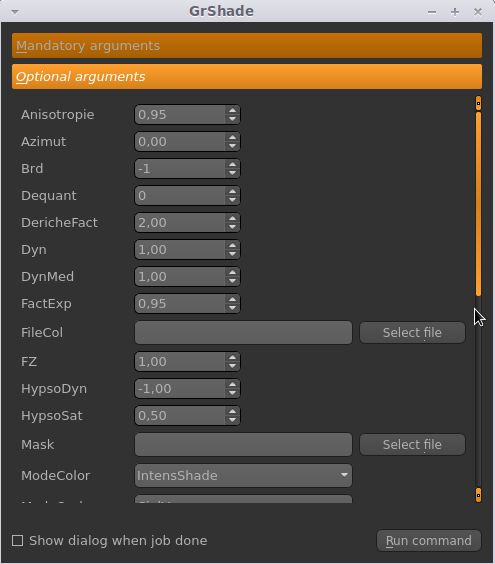
\includegraphics[width=87.31mm]{FIGS/Saisie/Visual.jpg}
\caption{Visual interface for command line tools}
\end{figure}

\subsection{Complex Tools}

For a more complex command, that requires arbitrary numbers of arguments, the command line
would not be manageable. For this command, it has been decided to use an {\tt XML} file
for specifying the parametrization. {\tt XML} has the following advantages:


\begin{itemize}
    \item it is a standard, with \UNCLEAR{current} specialized editor;
    \item the name tagging convention, although heavy for writing, make it easier to read;
    \item it allows textual description of attributed tree structures, which is
          exactly what is required for complex parametrization.
\end{itemize}

Here is an example for calling {\tt Apero}:

\begin{verbatim}
bin/Apero ../micmac_data/Ref-Apero/Test-Lion/AperoQuick.xml
\end{verbatim}

If you downloaded the data example as described in~\ref{Install}, you could have
a look at the {\tt AperoQuick.xml} file to see what it looks like. For all these
complex tools, that exit in an  XML file, there is a formal description of the
XML file that is correct from the syntactic point of view. These XML formal description
files are all  located in the {\tt include/XML\_GEN/} directory.
For example, the file {\tt include/XML\_GEN/ParamApero.xml} contains a formal
description of the XML files which are syntactically valid XML files for the
{\tt Apero} program.

How the formal files are used to specify the valid files is too complex
to describe it here. The mechanism is described in chapter~\ref{Mic:Tree:Match}.
Basically, the idea is that the parameter file
must be a sub-tree of the specification file satisfying some arity
constraints.


Generally, the {\tt XML} file can be modified using optional command line
arguments. For example, you can run one of the example data set with no
argument:

\begin{verbatim}
bin/MICMAC /home/mpd/micmac_data/Jeux1-Spot-Epi/Param-0-Epi.xml
\end{verbatim}

But if, for some reason, you want to start the computation directly
from the second step you shall add an optional argument and type:

\begin{verbatim}
bin/MICMAC /home/mpd/micmac_data/Jeux1-Spot-Epi/Param-0-Epi.xml  FirstEtapeMEC=2
\end{verbatim}


\subsection{Where Calling the Tools From (The Mandatory Working Directory)}

At the beginning of {\tt MicMac}, it was mandatory to run the file from the
{\tt micmac} directory. This is why in all the examples you will see
commands like {\tt bin/MICMAC \dots}. As I had a lot of complaints
about this not being very convenient, I have corrected this fact for most
of the tools. However, I do not guarantee that this has been corrected
everywhere. So if you encounter problems, you should try to run the file
from the {\tt micmac} directory.



%=======================================================================================================

\section{Data Organization and Communication}

When you want to use photogrammetric tools for complex tasks, there are a lot
of things about data organization that has to be specified to programs.
For example:

\begin{itemize}
   \item  at a given step, you want to orientate a certain subset of images of a
          project; so you need  to have the possibility to specify sets
          and subsets of files;

   \item  sometimes you will want to specify that if an image name is
          {\tt toto\_123.tif} or  {\tt toto\_0123.tif}  then the associated orientation is
          {\tt 123\_tata.xml}; so you need to have the possibility to specify the probably complex
          rules of computation that transform strings to strings;

   \item  sometimes you will want to specify that a matching process (for example
          tie points computation) must be executed between all pairs of images satisfying
          certain conditions; so  you need to have the possibility to specify relations
          (in the mathematical way).
\end{itemize}

All these tasks may be performed by a database management system. Although there
are some very efficient systems such as open source systems, this is not what I chose
for supporting this functionality (because I wanted my tools to stay relatively autonomous).
Maybe it was not a good choice, however it has to be assumed now.


The precise mechanism is quite complex and it is described in the chapter~\ref{Chap:NFS}.
The main ideas are:

\begin{itemize}
   \item there is a huge use of modern regular expressions to specify string sets and
         string manipulation. For example, the pattern {\tt Img([0-9]\{4\}).tif} will
         describe the name set beginning with {\tt Img}, followed by four digits and ending
         with {\tt .tif}. If one wants to specify that the file associated  to {\tt Img1234.tif}
         is {\tt Ori/1234-HH.xml}, there will be something like {\tt  Ori/\$1-HH.xml} associated
        to {\tt Img([0-9]\{4\}).tif}  (the meaning is that {\tt \$1}  is to be replaced by
          the first sub-expression between parenthesis);



   \item to facilitate the sharing of sets, transformations, relations \dots between programs,
         generally they are not manipulated directly. They are created in a common file and
         are given a name (or Key). The program refers to these objects by their key which
         facilitates name convention sharing. For example, if the transformation
         {\tt Img([0-9]\{4\}).tif $\rightarrow$  Ori/\$1-HH.xml} is to be used
         to describe the association between image and orientation, it  may be declared in
         the file {\tt MicMac-LocalChantierDescripteur.xml} under the key {\tt Key-Im2Ori},
         this key will then be used in {\tt Apero} for the creation of orientation file and in
         {\tt MicMac} for using the result of {\tt Apero};


     \item a lot of pre-existing conventions are automatically loaded by the tools, and
           for most of the cases these standard conventions should be sufficient.
\end{itemize}

\UNCLEAR{For example} %il n'y a pas d'exemple


%=======================================================================================================

\section{Existing Tools}


\label{Gen:ExTools}

The pipeline for transforming a set of images in a 3D model, and optionally
generating ortho-photo, is made essentially of four
"complex" tools:


\begin{itemize}
   \item {\tt \bf Pastis}. In fact, this tool is no more than an interface to the
         well known \SiftPP, distribution of {\tt Sift}, there is no algorithmic
         added value. Its advantage is to integrate the tie point generation
         in a way compatible with the global pipeline;

   \item {\tt \bf Apero} starts from tie points generated by {\tt \bf Pastis},
         and optional complementary measurements, and generates external and internal
         orientations compatible with these measurements;

   \item {\tt \bf MicMac} starts from orientation generated by {\tt \bf Apero} and
         computes image matching;


   \item {\tt \bf Porto}  starts from individual rectified images, that have been
         optionally generated by  {\tt \bf MicMac}, and generates a global ortho-photo;
         this tool is still in a very early stage.
\end{itemize}

There are several auxiliary tools that may be helpful for importing or
exporting data at different steps of this pipeline:


\begin{itemize}
   \item {\tt \bf BatchFDC} for batching a set of commands;

   \item {\tt \bf Casa} for computing analytic surface (cylinder \dots),
                        from points cloud, very early stage;

   \item {\tt \bf ClipIm} for clipping image;

   \item {\tt \bf ConvertIm} for some image conversion;

   \item {\tt \bf Dequant} for quantifying an image;

   \item {\tt \bf GrShade} for compute shading from depth image;

   \item {\tt \bf MapCmd} transforms a command working on a single file in a command
         working on a set of files;

   \item {\tt \bf CpFileVide}   to complete

   \item {\tt \bf MpDcraw}, an interface to the great {\tt dcraw} offering some low-level
         service useful for image matching;

   \item {\tt \bf MyRename} for image renaming, using modern regular expression and giving the possibility
         to integrate xif data in the new name, tricky but necessary in the existing pipeline;

    \item {\tt \bf Nuage2Ply}, a tool to convert depth map in point cloud;

   \item {\tt \bf SaisieMasq}, a user friendly (compared to others \dots) tool to create
         mask upon an image;

   \item {\tt \bf ScaleIm}, tool for scaling image;

   \item {\tt \bf ScaleNuage}, tool for scaling internal representation of point cloud;

   \item {\tt \bf tiff\_info}, tool for giving information about a tiff file;

   \item {\tt \bf to8Bits}, tool for converting $16$ or $32$ bit image in a $8$ bit image.

   \item {\tt \bf SupMntIm}, tool for generating a superposition of image and MNT in hypsometry
         and level curves.

   \item {\tt \bf PanelIm}. Gather images in a panel.
\end{itemize}









